\documentclass[11pt,a4paper]{article}

% ---------- PACKAGES ----------
\usepackage[margin=2.5cm]{geometry}   % reasonable page margins
\usepackage{graphicx}                 % \includegraphics
\usepackage{float}                    % H = “exactly here” placement
\usepackage{booktabs}                 % nicer tables
\usepackage{array}                    % custom table column widths
\usepackage[hidelinks]{hyperref}      % clickable refs, no coloured boxes
\usepackage{caption}                  % better caption formatting

\setlength{\parskip}{6pt}             % small breathing space between paragraphs

% -----------------------------------------------------------
%          D O C U M E N T
% -----------------------------------------------------------
\begin{document}
	
	% ------------------------- Title Page ---------------------
	\title{\textbf{E-Commerce Webshop Prototype\\UX Design Portfolio Report}}
	\author{Enrico Ebert \and Kristian Popov \and Glison Doci \and Orik Mazreku}
	\date{\today}
	\maketitle
	\thispagestyle{empty}
	\newpage
	
	% -------------------------- Contents ----------------------
	\setcounter{tocdepth}{2}
	\tableofcontents
	\newpage
	
	% ==========================================================
	\section{Project Overview}
	Our e-commerce webshop delivers a \emph{simple, modern, and fully responsive} shopping experience. Essential features—product search, category filtering, and a shopping cart—are complemented by smart extras such as a light/
	-mode toggle.
	
	\subsection*{Target Users}
	\begin{itemize}
		\item \textbf{Regular Shoppers} browsing on laptops or smartphones.
		\item \textbf{Store Administrators} managing catalogue and user data.
	\end{itemize}
	
	\subsection*{Application Goals}
	\begin{itemize}
		\item Clean, intuitive UI and navigation.
		\item Fast product search and category filtering.
		\item Secure account creation and sign-in.
		\item Complete cart and checkout flow.
		\item Admin panel for catalogue and order management.
		\item Light/dark-mode toggle.
		\item Fully responsive grid down to 320 px.
	\end{itemize}
	
	% ==========================================================
	\section{Key Features}
	\begin{itemize}
		\item \textbf{Product Search \& Filters} — keyword, category, price.
		\item \textbf{Shopping Cart} — add, update, remove items.
		\item \textbf{Checkout} — multi-step form, confirmation.
		\item \textbf{Responsive Design} — fluid grid.
		\item \textbf{Light/Dark Mode} toggle.
		\item \textbf{User Accounts}, \textbf{Admin Dashboard}, \textbf{Discount Codes} (nice-to-have).
	\end{itemize}
	
	% ==========================================================
\section{User Interface Design}

% =======================================================
% 1) HOME SCREEN  ---------------------------------------
% =======================================================
\subsection{Home Screen}

\begin{figure}[H]
	\centering
	\includegraphics[width=\linewidth]{Home_Figma.png}%
	\caption{Home screen in light mode .}
	\label{fig:ui-home}
\end{figure}

\paragraph{Explanation}%
The home page follows a classic information funnel: brand section~$\rightarrow$ value
proposition~$\rightarrow$ featured category. A single call-to-action
(*“Shop Now”*) avoids decision fatigue on first contact.  
All interactive controls (search, cart) are reachable within one
tap.

\begin{table}[H]
	\centering
	\caption{Home screen – elements and rationale}
	\label{tab:home-elements}
	\begin{tabular}{p{0.30\linewidth} p{0.60\linewidth}}
		\toprule
		\textbf{Design element} & \textbf{Purpose \& rationale} \\ \midrule
		Persistent top-bar      & Immediate access to search \& cart.\\
		Hero banner             & Communicates value proposition in one glance; accent colour draws the eye.\\
		Category carousel       & Promotes bestselling category; horizontal swipe invites mobile interaction.\\
		
		\bottomrule
	\end{tabular}
\end{table}
\subsection{Category Drawer (Hamburger / Desktop “Categories”)}

\begin{figure}[H]
	\centering
	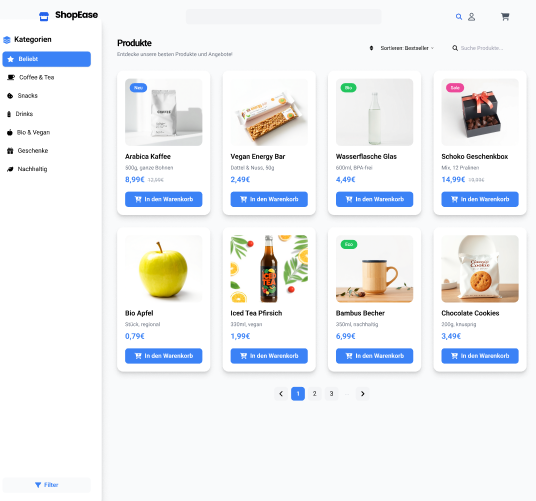
\includegraphics[width=\linewidth]{categories_Figma.png}%
	\caption{Off-canvas category drawer; mobile and desktop share the same component.}
	\label{fig:ui-category-drawer}
\end{figure}

\paragraph{Explanation}%
The drawer offers an identical filtering experience on both breakpoints:
a hamburger icon triggers it on mobile, while a “Categories” pill does so on
desktop. The underlying product grid is dimmed but remains in place, giving
immediate visual feedback when a category is selected.

\begin{table}[H]
	\centering
	\caption{Category drawer – elements and rationale}
	\label{tab:category-elements}
	\begin{tabular}{p{0.30\linewidth} p{0.60\linewidth}}
		\toprule
		\textbf{Design element} & \textbf{Purpose \& rationale} \\ \midrule

		Hamburger icon (mobile) & Saves horizontal space; familiar pattern. \\
		“Categories” pill (desktop) & reveals drawer on click. \\
		Accordion list          & Supports deep hierarchies without scrolling fatigue. \\
	
		\bottomrule
	\end{tabular}
\end{table}
% =======================================================
% 2) PRODUCT LIST SCREEN  -------------------------------
% =======================================================
\subsection{Product List Screen}

\begin{figure}[H]
	\centering
	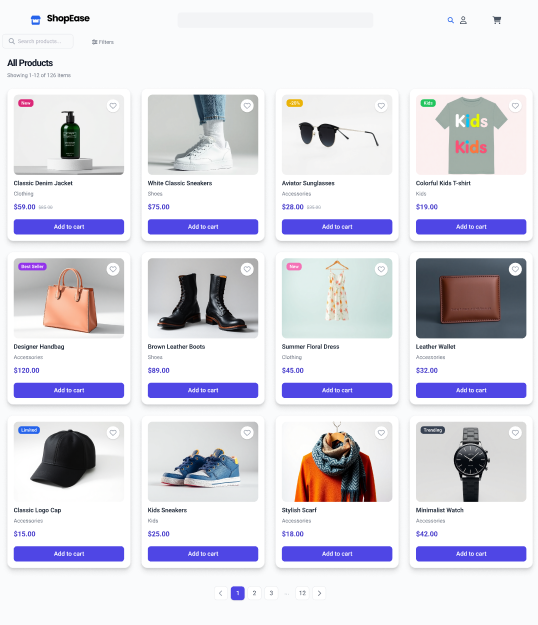
\includegraphics[width=\linewidth]{Product_List_Figma.png}%
	\caption{Product grid with search bar and category filter.}
	\label{fig:ui-products}
\end{figure}

\paragraph{Explanation}%
Users can search \emph{and/or} filter without leaving the page.  
The responsive grid keeps card proportions intact  focusable
cards maximise tap targets on touch devices.

\begin{table}[H]
	\centering
	\caption{Product list – elements and rationale}
	\label{tab:product-elements}
	\begin{tabular}{p{0.30\linewidth} p{0.60\linewidth}}
		\toprule
		\textbf{Design element} & \textbf{Purpose \& rationale} \\ \midrule
		Secondary navigation    & Lets users pivot between catalogue views (SPA routing).\\
		Search field            & Supports goal-oriented discovery; full-width on desktop, icon on mobile.\\
		Category dropdown       & Progressive narrowing while preserving context; default “Show all” reveals filter state.\\
	
	
		\bottomrule
	\end{tabular}
\end{table}


	
	% ==========================================================
	\section{Navigation Flow}

	% ==========================================================
	\section{Design Decisions \& Rationale}
	....
	% ==========================================================
	\section{Responsiveness \& Accessibility}
	Fluid CSS grid, break-points 1024 / 768 / 480 px, keyboard navigation, aria-labels, reduced-motion support.
	
	% ==========================================================
	\section{Acknowledgment of AI Technologies}
	Document drafted with GPT-4o assistance; final content reviewed and refined by the authors.
	
	% ==========================================================
	\section{Conclusion}
	This portfolio meets all assignment requirements and provides a clear blueprint for development.
	
	% ==========================================================
	\appendix
	\section{Detailed Use-Case Flows}\label{app:usecases}
	(See attached PDF for step-by-step flows.)
	
\end{document}